\chapter{Send e Receive}

\example{
\begin{itemize}
\item \texttt{mailman.c}
\item \texttt{postbox.c}
\end{itemize}
}

A comunicação do PD com \externals nem sempre é feita por conexões explícitas.
Outra maneira de permitir a comunicação entre objetos é por meio de \texttt{send} e
\texttt{receive}.
Esta opção está presente em objetos gráficos como o \texttt{toggle} e \texttt{bang}, por exemplo.
Para utilizar tal tipo de mensagem é necessário definir o nome da mensagem que
o objeto pretende receber.

\begin{figure}[h!]
\centering
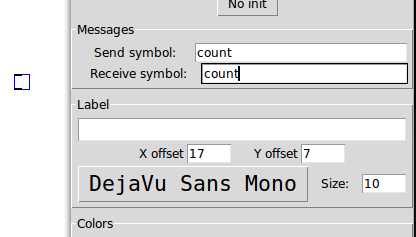
\includegraphics[scale=\Mysize]{toggle}
\caption{Exemplo de configuração de um \texttt{toggle} para envio e recebimento de mensagens}
\end{figure}

Neste capítulo vamos verificar como enviar e receber mensagens.
Para maiores informações quanto a este tipo de mensagens, consulte o código dos
objetos send e receive no repositório do PD\footnote{
\url{https://github.com/libpd/libpd/blob/master/pure-data/src/x_connective.c}
}.

% -----+-----+-----+-----+-----+-----+-----+-----+-----+-----+-----+-----+-----+
%      |     |     |     |     |     |     |     |     |     |     |     |     |
% -----+-----+-----+-----+-----+-----+-----+-----+-----+-----+-----+-----+-----+
\section{Enviando mensagens}

O envio de utiliza funções distintas dependendo do tipo da mensagem a ser enviada.
As funções para envio de mensagem são:

\begin{itemize}
\item \texttt{pd\_bang(t\_pd *x)}
\item \texttt{pd\_float(t\_pd *x, t\_float f)}
\item \texttt{pd\_symbol(t\_pd *x, t\_symbol *s)}
\item \texttt{pd\_pointer(t\_pd *x, t\_gpointer *gp)}
\item \texttt{pd\_list(t\_pd *x, t\_symbol *s, int argc, t\_atom *argv)}
\item \texttt{typedmess(t\_pd *x, t\_symbol *s, int argc, t\_atom *argv)}
\end{itemize}

A última função, que não define tipo para a mensagem, é uma espécie de ``anything''.
O primeiro parâmetro para todas as funções define o nome da mensagem e pode ser
conseguido de um \texttt{symbol} em seu atributo \texttt{s\_thing}.

No exemplo mailman.c, o objeto envia mensagens para um conjunto de diferentes 
seletores recebidos como parâmetro.
As mensagens são do tipo \texttt{bang} e enviadas quando o objeto recebe um \texttt{bang}.

\begin{lstlisting}[caption=Envio de mensagens bang por send]
void mailman_bang(t_mailman *x){
   int i = 0;
   for(; i < x->argc ; i++){
      if (x->messages[i]->s_thing)
         pd_bang(x->messages[i]->s_thing);
   }
}
\end{lstlisting}

O resultado pode ser visto na Figura \ref{fig:mailman}.
\begin{figure}[h!]
\centering
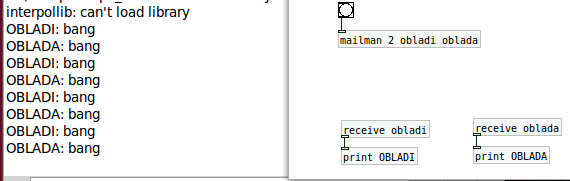
\includegraphics[scale=\Mysize]{mailman}
\caption{Envio de mensagens por send}
\label{fig:mailman}
\end{figure}


% -----+-----+-----+-----+-----+-----+-----+-----+-----+-----+-----+-----+-----+
%      |     |     |     |     |     |     |     |     |     |     |     |     |
% -----+-----+-----+-----+-----+-----+-----+-----+-----+-----+-----+-----+-----+
\section{Receive}

O recebimento de mensagens junto ao PD ocorre por meio de uma função
\texttt{bind} com o o símbolo esperado.

\begin{itemize}
   \item \texttt{pd\_bind(t\_pd *x, t\_symbol *s)}
   \item \texttt{pd\_unbind(t\_pd *x, t\_symbol *s)}
\end{itemize}

Nestas funções, o primeiro parâmetro é seu objeto e o segundo parâmetro é a
mensagem que esperada receber.

\begin{lstlisting}[caption=Exemplo de objeto que recebe várias mensagens]
void * postbox_new(t_symbol *s, int argc, t_atom *argv){
   t_postbox *x = (t_postbox *) pd_new(postbox_class);
   int i = 0;
   int counter = 0;
   for(; i < argc ; i++){
      if((argv + i)->a_type == A_SYMBOL)
         counter++;
   }
   x->messages = getbytes(counter * sizeof(t_symbol *));
   counter = 0;
   for(i = 0; i < argc ; i++){
      if((argv + i)->a_type == A_SYMBOL){
         x->messages[counter] = atom_getsymbol(argv + i);
         pd_bind(&x->x_obj.ob_pd, x->messages[counter]);
         counter++;
      }
   }
//   pd_bind(&x->x_obj.ob_pd, gensym("#key"));
//   pd_bind(&x->x_obj.ob_pd, gensym("#keyname"));
//   pd_bind(&x->x_obj.ob_pd, gensym("#keyup"));
   x->argc = counter;
   x->x_outlet = outlet_new(&x->x_obj, gensym("bang"));
   return (void *) x;
}
\end{lstlisting}

É importante que, no destrutor do objeto, a ligação seja desfeita para evitar
que o PD aborte ao tentar enviar uma mensagem para um objeto que não existe mais.
Isto é feito pela função \texttt{unbind}, apresentada abaixo.

\begin{lstlisting}[caption=Desvinculando o objeto com a mensagem no destrutor]
void postbox_destroy(t_postbox *x) {
   outlet_free(x->x_outlet);
   int i = 0;
   for(; i < x->argc ; i++){
      pd_unbind(&x->x_obj.ob_pd, x->messages[i]);
   }
//   pd_unbind(&x->x_obj.ob_pd, gensym("#key"));
//   pd_unbind(&x->x_obj.ob_pd, gensym("#keyname"));
//   pd_unbind(&x->x_obj.ob_pd, gensym("#keyup"));
}
\end{lstlisting}


Uma vez associado o recebimento de um determinado símbolo, é necessário definir
qual método será chamado para cada tipo de mensagem recebida.
A definição destes métodos é similar a definição dos inlets ativos.
É ideal que um objeto que possua um receive possua métodos para receber todos
os tipos de mensagens do PD, mesmo que tais métodos não sejam utilizados.

\begin{lstlisting}[caption=Associando métodos para receber mensagens]
void postbox_list_method(t_postbox *x, t_symbol *s, int argc, t_atom *argv){
   post("list %s", atom_getsymbolarg(1, argc, argv)->s_name);
}

void postbox_setup(void) {
   postbox_class = class_new(gensym("postbox"),
      (t_newmethod) postbox_new, // Constructor
      (t_method) postbox_destroy, // Destructor
      sizeof (t_postbox),
      CLASS_NOINLET,
      A_GIMME,
      0);//Must always ends with a zero

   class_addbang(postbox_class, postbox_bang_method);
   class_addfloat(postbox_class, postbox_float_method);
   class_addlist(postbox_class, postbox_list_method);
}
\end{lstlisting}

Note que este objeto (postobox.c) não possui \texttt{inlets} e por isto tais métodos
só serão usados para mensagens.
Caso o mesmo possua \texttt{inlets}, o tratamento de mensagens recebidas pelo \texttt{inlet} ou
por \texttt{receive} será exatamente o mesmo, o que é muito bacana.


% -----+-----+-----+-----+-----+-----+-----+-----+-----+-----+-----+-----+-----+
%      |     |     |     |     |     |     |     |     |     |     |     |     |
% -----+-----+-----+-----+-----+-----+-----+-----+-----+-----+-----+-----+-----+
\section{Indo além disto}

Entender como receber mensagens enviadas pelo PD ajudará a entender como trocar
mensagens entre um objeto PD em C e sua interface em tcl/tk.
Além disto, é possível receber e enviar mensagens padrões do PD, como movimentos
de teclado, entradas MIDI e assim por diante.

Com isto, é possível desenvolver um \external que envia eventos de teclado ou
que recebe eventos de teclado diretamente.

Alguns exemplos de mensagens internas do PD que são trocadas por \texttt{send} /
\texttt{receive} são:

\begin{itemize}
   \item Eventos de teclado\footnote{Retirados de: \url{https://github.com/libpd/libpd/blob/master/pure-data/src/x_gui.c}}
   \begin{itemize}
      \item \texttt{\#key}
      \item \texttt{\#keyup}
      \item \texttt{\#keyname}
   \end{itemize}
   \item Eventos MIDI\footnote{Retirados de: \url{https://github.com/libpd/libpd/blob/master/pure-data/src/x_midi.c}}
   \begin{itemize}
      \item \texttt{\#midiin}
      \item \texttt{\#sysexin}
      \item \texttt{\#notein}
      \item \texttt{\#ctlin}
      \item \texttt{\#pgmin}
      \item \texttt{\#bendin}
      \item \texttt{\#touchin}
      \item \texttt{\#polytouchin}
      \item \texttt{\#midiclkin}
      \item \texttt{\#midirealtimein}
      \item \texttt{\#midiclkin}
      \item \texttt{\#midiclkin}
   \end{itemize}
\end{itemize}

\todo{Acho que seria bacana alguns exemplos disto tudo...}
